%!TEX root = ../dokumentation.tex

\chapter{Concept}\label{cha:Concept}
This chapter outlines the concept and the architecture of \ac{Synplifier}. In section \ref{sec:ConceptApproach} a general approach to build \ac{Synplifier} is outlined and in section \ref{sec:ConceptRequirements} resulting requirements \ac{Synplifier} needs to meet are described.
Section \ref{sec:ConceptOverview} introduces into the architecture of \ac{Synplifier} and its components.
The sections following section \ref{sec:ConceptOverview} describe the concept of each component that is developed.

\section{Approach}\label{sec:ConceptApproach}

In order to decompose the full \ac{TPTP} syntax into smaller sub-syntaxes extracting desired sub-syntaxes by selecting a new start symbol and disabling undesired productions is proposed.
The idea is to process the full \ac{TPTP} syntax in multiple stages.
These stages include parsing the syntax into a structured internal representation and presenting it to the user in order to define undesired productions and the start symbol. To extract the sub-syntax, we introduce a recursive algorithm that checks which productions are still reachable and extracts all reachable
productions.

\section{Requirements}\label{sec:ConceptRequirements}

The following section outlines requirements of \ac{Synplifier}. Requirements are numbered and split into three categories: 

\begin{itemize}
\item Requirements concerning the GUI are marked by a $G$
\item Requirements concerning the Command-line interface are marked by a $C$
\item General requirements concerning \ac{Synplifier} are marked by a $R$
\end{itemize}

The requirements are described using capitalized keywords like MUST or SHOULD following \cite{Bradner.1997}.

\subsubsection{[G1]}\label{G1}
\ac{Synplifier} MUST provide a GUI.
\subsubsection{[G2]}\label{G2}
\ac{Synplifier} MUST provide the possibility for the user to import a \ac{TPTP} syntax file into the GUI by specifying a \ac{TPTP} syntax file path and a desired start symbol. 
\subsubsection{[G3]}\label{G3}
The imported syntax MUST be displayed in the GUI. This includes displaying by the syntax defined productions as well as comments that are associated with these productions.
\subsubsection{[G4]}\label{G4}
The user MUST be able to select a new start symbol in order to generate a sub-syntax.
\subsubsection{[G5]}\label{G5}
The user MUST be able to select which productions should be blocked in order to generate a sub-syntax.
\subsubsection{[G6]}\label{G9}
\ac{Synplifier} MUST provide the functionality for the user to import a control file into the GUI by specifying a control file path. 
\subsubsection{[G7]}\label{G7}
After importing a control file, selections are set according to the control file content in the GUI.
\subsubsection{[G8]}\label{G8}
\ac{Synplifier} MUST provide the functionality to display a generated sub-syntax in the GUI.
\subsubsection{[G9]}\label{G9}
The user MUST be able to export a control file based on the users start symbol selection (G2) and blocked productions selection (G3) in a .txt-format.
\subsubsection{[G10]}\label{G10}
\ac{Synplifier} MUST provide the functionality in the GUI for the user to export a generated sub-syntax to .txt format by specifying a file path.
\subsubsection{[C1]}\label{C1}
\ac{Synplifier} MUST provide a command-line interface.
\subsubsection{[C2]}\label{C2}
The command-line interface MUST provide the functionality to extract a sub-syntax with the user specifying the \ac{TPTP} syntax file and control file path.
\subsubsection{[C3]}\label{C3}
The extracted sub-syntax is saved in .txt format at a file path that has been specified by the user.
\subsubsection{[C4]}\label{C4}
The command-line interface MUST provide help information which describe all command-line parameters.
\subsubsection{[R1]}\label{R1}
When generating a sub-syntax comments referring to rules that are present in the reduced syntax SHOULD be maintained in the sub-syntax.
\subsubsection{[R2]}\label{R2}
Output \ac{TPTP} sub-syntaxes SHOULD be compatible to the automated parser generator for the \ac{TPTP} language \cite{VS06}.
\subsubsection{[R3]}\label{R3}
A generated sub-syntax MUST only contain terminating and reachable symbols.


%nonfunctional requirements
%
%Furthermore, \ac{Synplifier} is able to import a control file and extract a sub-syntax based on this control file instead of extracting a sub-syntax based on a user's selection of blocked productions.
%%The new sub-syntax can be exported to .txt format.
%Also, comments referring to the remaining productions are kept and comments referring to productions that were discarded are not be included in the sub-syntax.
%\ac{Synplifier} also provides a console interface. This interface accepts a \ac{TPTP} syntax file and a control file and output the sub-syntax described in the control file. It is possible to specify the output path and filename.

\section{Overview}\label{sec:ConceptOverview}
Figure \ref{fig:ConceptProcessSublanguage} outlines the procedure of extracting a sublanguage of the \ac{TPTP} language.
The first task is to import the \ac{TPTP} syntax file and extract the tokens inside that file using the lexer.
The next phase is for the parser to create a data structure from the tokens, also checking if the syntax in the syntax file was correct.
Then, a graph representing the imported \ac{TPTP} syntax is built.\\
This graph is subject to manipulation by disabling certain transitions or selecting a new start symbol in the following phase.
This includes computation of the remaining reachable and terminating syntax.
That new graph represents the syntax of the extracted sub-language.
To make this syntax usable, lastly the syntax has to be output, based on the new graph, in the same format as the original syntax.
\begin{figure}[H]
\tikzstyle{decision} = [ diamond, draw, fill=blue!10, text width=4.5em, text badly centered, node distance=2cm, inner sep-0pt]  
\tikzstyle{block} = [ rectangle, draw, fill=blue!10, text width=4.5em, text badly centered, rounded corners, minimum height=4em]  
\tikzstyle{line} = [ draw, -latex']  
\tikzstyle{terminator} = [rectangle, draw, fill=blue!10, text width=4.5em, text badly centered, rounded corners, minimum height=4em]  
\begin{center}
\begin{tikzpicture}[node distance=3cm, auto]  
  \node [terminator]  (lex)  {Import of syntax file and lexing};  
  \node [block, right of=lex]  (pars) {Parsing};  
  \node [block, right of=pars] (ggg) {Grammar graph generation}; 
  \node [block, right of=ggg] (ggm) {Grammar graph modification}; 
   \node [block, right of=ggm] (go) {Grammar output};  
  \path [line] (lex)  -- (pars);  
  \path [line] (pars) -- (ggg);  
  \path [line] (ggg) -- (ggm); 
  \path [line] (ggm) -- (go);  
\end{tikzpicture}
\end{center}
\caption{Procedure of extracting a sublanguage}
\label{fig:ConceptProcessSublanguage}
\end{figure}

\subsection{Proposed architecture}\label{sec:ConceptProposedArchitecture}
The proposed architecture for \ac{Synplifier} consists of seven components:
\begin{itemize}
\item A lexer for extracting tokens from the \ac{TPTP} syntax
\item A parser for creating a data structure from the tokens
\item A graph builder for building a graph out of the parsers data structure and manipulating this graph
\item A graphical user interface
\item A console interface 
\item An input module that imports the \ac{TPTP} syntax
\item An output module that exports extracted sub syntaxes to local storage
\end{itemize}

%The architecture of the \ac{Synplifier} should take the procedure of extracting a sublanguage (section \ref{sec:ConceptOverview}) into consideration.
%From that, five main components can be identified:
%An import module responsible for importing the \ac{TPTP} syntax from a file;
%A lexer for extracting tokens from the language specification; A parser for creating a data structure from the tokens;
%A graph builder and manipulator;
%An export module for exporting the graph in a text representation corresponding to the original language specification.\\
%In addition to the components that provide the main functionality a graphical user interface and a console interface for user convenience is desired.

Figure \ref{fig:ConceptArchitectureOverview} contains a high-level UML diagram describing the architecture of \ac{Synplifier}. The user interacts either with the \textit{Console} or \textit{View} class. The \textit{Console} class provides the command-line interface and the \textit{View} class provides the GUI. Both have a reference on \textit{Input} and \textit{Output} for reading from and writing to files. They also have a reference on the \textit{TPTPGraphBuilder} class. This class is responsible for building a grammar graph and extracting sub-syntaxes by graph manipulation. For that, lexing and parsing are necessary. The \textit{TPTPGraphBuilder} uses the \textit{Parser} class for getting a \ac{TPTP} syntax representation and the \textit{Parser} uses the \textit{Lexer} to extract the tokens from a \ac{TPTP} syntax file.
\begin{figure}[H]
\centering
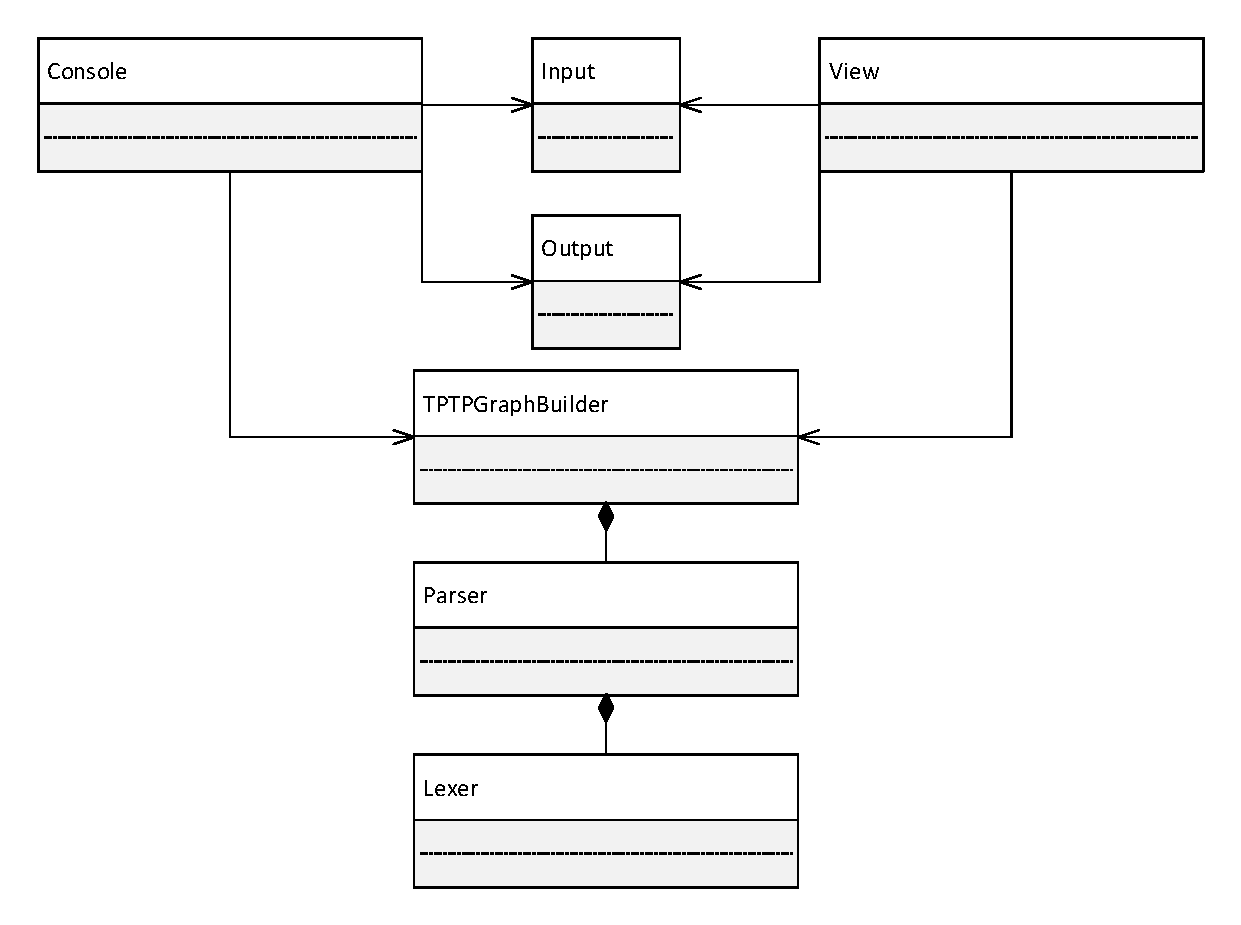
\includegraphics[width=1\textwidth]{images/Concept_UML_Architecture_Overview.pdf}
\caption{UML diagram of the architecture of \ac{Synplifier}}
\label{fig:ConceptArchitectureOverview}
\end{figure}

\section{Lexer}\label{sec:ConceptLexer}
The lexer is responsible for extracting tokens from the \ac{TPTP} syntax file. Using \ac{PLY} a lexer can be generated by specifying tokens using regular expressions.\\
In order to find elementary tokens the \ac{TPTP} syntax has been analyzed and regular expressions that precisely describe these tokens have been defined.

The standard \ac{EBNF} only uses one production symbol ($"::="$).
In the \ac{TPTP} syntax the standard production symbol is used for syntactic rules.
Additional symbols for semantic, lexical and character-macro rules have been added. Semantic rules describe rules whose left-hand side is already part of a syntactic rules but from which only a subset makes semantic sense. Any further rules that are reached from the nonterminal symbols on the right-hand side of a semantic rule are semantic rules as well. Lexical rules are rules that produce tokens. Character-macro rules are rules that define regular expressions for the tokens.
The following table contains the production symbols for grammar (syntactic rules), strict (semantic rules), token (lexical rules) and macro (character-macro rules) rule types used in the \ac{TPTP} syntax.

\begin{table}[H]
\centering
\renewcommand{\arraystretch}{1}
\caption{\ac{TPTP} language rule types \cite{VS06}}
\begin{tabular}{ll}
\textbf{Symbol} & \textbf{Rule Type}\\\hline
::= & Grammar\\
:== & Strict\\
::- & Token\\
::: & Macro\\
\end{tabular}
\label{tbl:ConceptTPTPProductionSymbols}
\end{table}

The following paragraph introduces the tokens that are recognized by the lexer. Tokens are written in bold.

Following standard \ac{BNF}, \textbf{nonterminal} symbols are enclosed by the \textless\; and \textgreater \;symbol.
In between there can be any arbitrary sequence of alphanumerical characters and underscores.

A \textbf{terminal symbol} does not have any special notation and can be any sequence of characters excluding whitespace characters that is not matched to any other token.

There are four \textbf{expression} token types (one for each rule type).
\textbf{Expressions} are defined as a nonterminal symbol followed by a production symbol (::= for grammar, ::- for token, :== for strict, ::: for macro rule type).
The nonterminal symbol and the following production symbol are selected to be a single token and are not identified as two separate tokens to clearly identify the start of a new rule and therefore avoid ambiguity while parsing.
The listing below features two tokens, a grammar expression and a nonterminal symbol.
\begin{lstlisting}[caption= Rule example]
<formula_role>         ::= <lower_word>
\end{lstlisting}

A \textbf{comment} is defined as the start of a new line, a percentage sign, arbitrary characters and ends with a newline character.
The percentage sign when used as terminal symbol is embedded in square brackets and can therefore never be the first character of a new line.

Additional tokens are the meta-symbols including \textbf{open} $"("$ and \textbf{close parentheses} $")"$, \textbf{open} $"["$ and \textbf{close square brackets} $"]"$, asterisks $"*"$ called \textbf{repetition symbols} and vertical bars $"\mid"$ called \textbf{alternative symbols}.

In PLY it is possible to declare characters that should be ignored. This means that the characters are ignored in the input stream of the lexer. However, if one of those characters are part of a regular expression of a token they are not ignored and will be used for token matching. In this project tabs, white spaces and newline characters are ignored as they do not have any special meaning other than providing better readability. With exception of the comment token, the information about newline characters is not relevant due to rules being defined over multiple lines, which can be seen in the listing below.
\begin{lstlisting}[caption= Example of rules defined over multiple lines]
<annotated_formula>  ::=    <thf_annotated> | <tff_annotated> |
                            <tcf_annotated> | <fof_annotated> |
                            <cnf_annotated> | <tpi_annotated>
\end{lstlisting}

\section{Parser}\label{sec:ConceptParser}
The parser takes the tokens from the lexer as input and creates a data structure that represents the structure of the \ac{TPTP} syntax.

Figure \ref{fig:ConceptParserFlow} outlines the responsibilities of the parser component and the sequence of its sub-functions.
First, the tokens generated by the lexer need to be parsed and based on that the data structure representing the \ac{TPTP} syntax is to be created.
The rules in the data structure have to be numbered, to maintain the correct order for output, after creating the grammar tree in the next step.

In the \ac{TPTP} syntax square brackets not necessarily denote that an expression is optional, which is the case in traditional \ac{EBNF}.
In token and macro rules they denote that an expression is optional and in grammar and strict rules square brackets are terminals.
Therefore, disambiguation of square brackets is necessary.
\begin{figure}[H]
\tikzstyle{decision} = [ diamond, draw, fill=blue!10, text width=4.5em, text badly centered, node distance=2cm, inner sep-0pt]  
\tikzstyle{block} = [ rectangle, draw, fill=blue!10, text width=5em, text badly centered, rounded corners, minimum height=4em]  
\tikzstyle{line} = [ draw, -latex']  
%\tikzstyle{terminator} = [ draw, ellipse, fill=red!20, node distance=3cm, minimum height=2em]
\tikzstyle{terminator} = [rectangle, draw, fill=blue!10, text width=5em, text badly centered, rounded corners, minimum height=4em]  
\begin{center}
\begin{tikzpicture}[node distance=3cm, auto]  
  \node [terminator]  (start)  {Parse tokens};  
  \node [block, right of=start]  (number) {Number rules};  
  \node [block, right of=number] (disambigue) {Disambigue square brackets}; 
  \node [block, right of=disambigue] (return) {Return result}; 
 
  \path [line] (start)  -- (number);  
  \path [line] (number) -- (disambigue);  
  \path [line] (disambigue) -- (return); 
\end{tikzpicture}
\end{center}
\caption{Parsing procedure}
\label{fig:ConceptParserFlow}
\end{figure}

\subsection{Data structures and data types}\label{sec:ConceptParserDataStructure}

When using the \ac{PLY} parser generator, production rules and data types that store the data of the \ac{TPTP} syntax have to be defined in order to generate the parser. Data types are implemented using Python classes. In the following production rules are written in italic and data types are written in bold.

A \textit{t\textunderscore symbol\textunderscore  production} rule implies a \textbf{t\textunderscore symbol} that has two attributes. These are the value of the terminal symbol token it represents and additionally a production property.

A production property can take two values and denotes whether a t\textunderscore  symbol is embedded in square brackets or not. In the production rules a terminal symbol token, either embedded in square brackets or without brackets, can be derived from a t\textunderscore  symbol\textunderscore  production. Asterisk and vertical bar tokens embedded in square brackets can be derived from a t\textunderscore  symbol production as well. 

Analogue to the t\textunderscore symbol data type, the \textbf{nt\textunderscore  symbol} also has the value of the non-terminal symbol token as an attribute. 

Due to the similarities of \textbf{t\textunderscore symbol} and \textbf{nt\textunderscore  symbol} they are inherited from the same base class \textbf{symbol} that can be seen in figure \ref{fig:ConceptSymbolsClassDiagram}.

\begin{figure}[H]
\centering
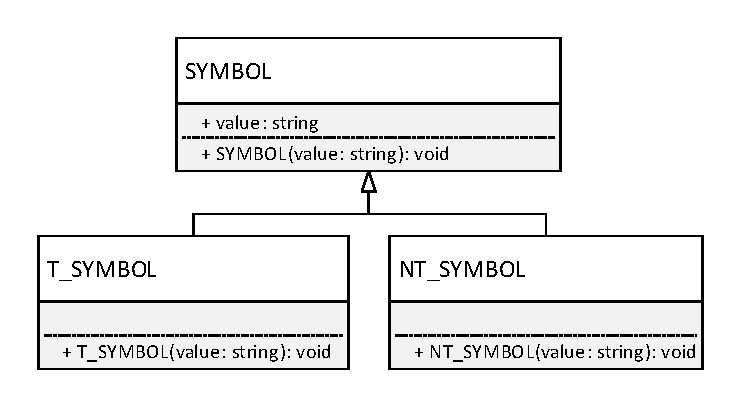
\includegraphics[width=.8\textwidth]{images/Concept_uml_data_types_symbols.pdf}
\caption{Symbol data type UML class diagram}
\label{fig:ConceptSymbolsClassDiagram}
\end{figure}

A \textbf{rule} consists of an expression token, a production list and a position.
The position denotes at which position in the TPTP syntax the rule was listed.
This information is needed to maintain the original order of the rules when printing the reduced syntax.
For each rule type there is a data type.
This means that \textbf{grammar, token, strict} and \textbf{macro rule} data types are introduced. They inherit from the same base class \textbf{rule} which can be seen in figure \ref{fig:ConceptRulesClassDiagram}.
Listing \ref{lst:ConceptParserGrammarExpression} contains an example of a line in a \ac{TPTP} syntax file that is represented by the grammar rule data type.
The nonterminal symbol name which is produced is <$tff \textunderscore formula$>.  The production list consists of two productions, as can be seen in the listing.
\begin{lstlisting}[basicstyle=\scriptsize	,caption= Grammar expression,label= lst:ConceptParserGrammarExpression]
<tff_formula>          ::= <tff_logic_formula> | <tff_atom_typing
\end{lstlisting}

\begin{figure}[H]
\centering
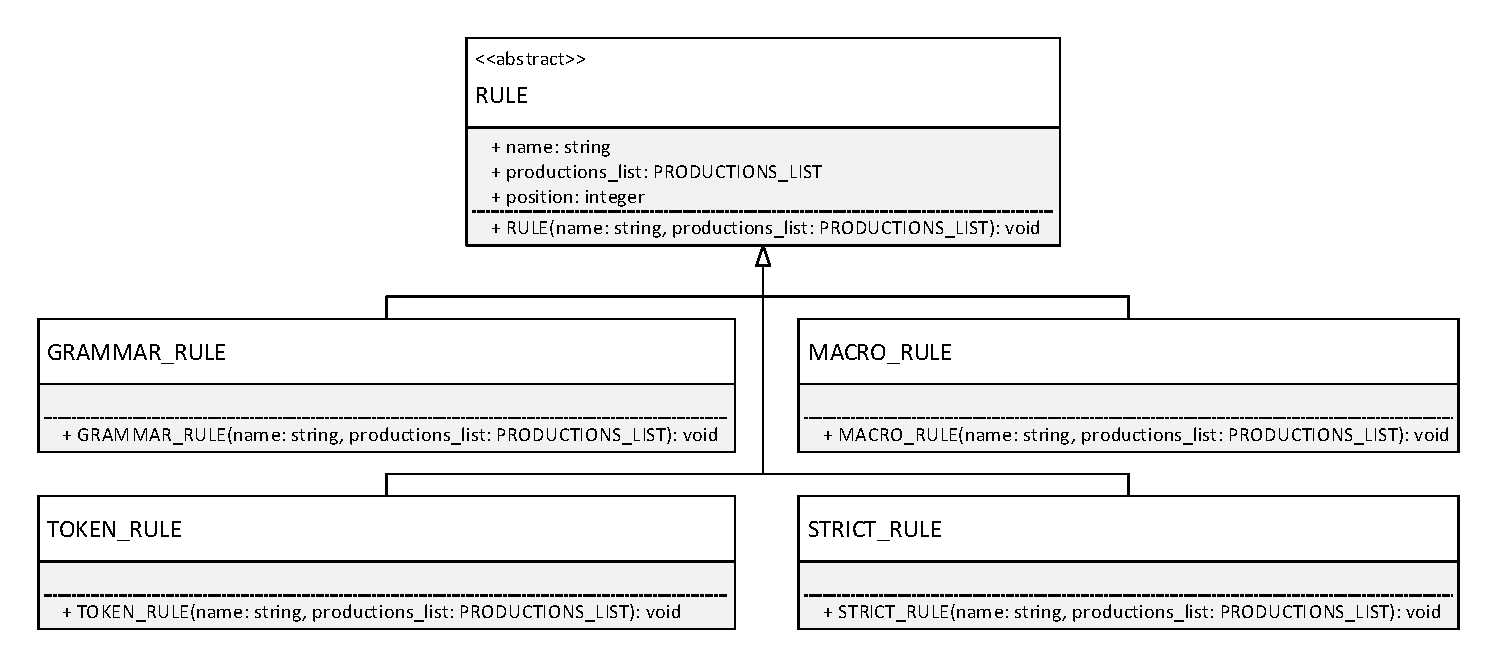
\includegraphics[width=1\textwidth]{images/Concept_uml_data_types_rules.pdf}
\caption{Rule data type UML class diagram}
\label{fig:ConceptRulesClassDiagram}
\end{figure}

A \textbf{comment\textunderscore block} is a list of consecutive comment lines. Comment lines can also be extended after initialising a comment block. Figure \ref{fig:ConceptCommentBlockClassDiagram} shows the UML denotation of a comment block.

\begin{figure}[H]
\centering
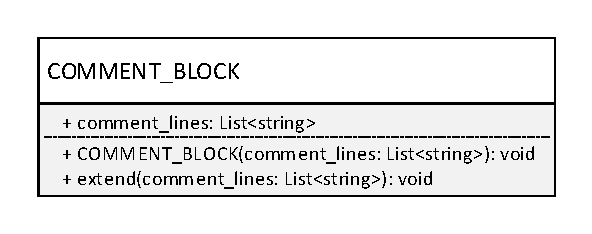
\includegraphics[width=.5\textwidth]{images/Concept_uml_data_types_comment_block.pdf}
\caption{Comment block data type UML class diagram}
\label{fig:ConceptCommentBlockClassDiagram}
\end{figure}


A \textbf{production\textunderscore element} is either a t\textunderscore symbol\textunderscore production or a nt\textunderscore symbol. Therefore it has an instance of \textbf{symbol} as an attribute which can be seen in figure \ref{fig:ConceptProductionElementClassDiagram}. Additionally, a production element has a production property that is shown in figure \ref{fig:ConceptProductionPropertyClassDiagram}.
The production property can take one of three values and denotes whether a production is optional, can be repeated multiple times or does not have any special property.
In the original TPTP syntax file, the property is represented by square brackets or the repetition symbol. A production element can also only consist of square brackets (see Figure \ref{fig:ImplementationParsing}).

\begin{figure}[H]
\centering
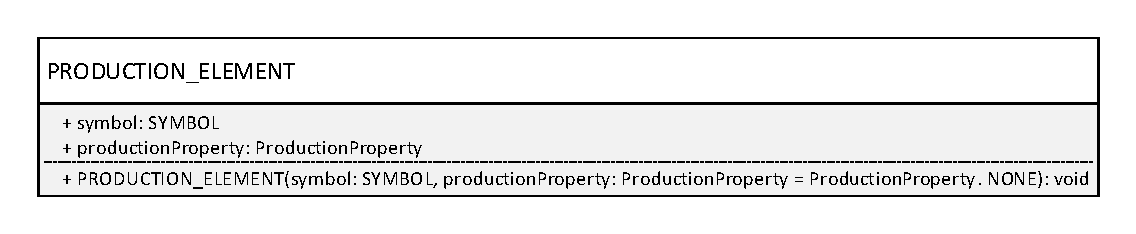
\includegraphics[width=.8\textwidth]{images/Concept_uml_data_types_production_element.pdf}
\caption{Production element data type UML class diagram}
\label{fig:ConceptProductionElementClassDiagram}
\end{figure}

\begin{figure}[H]
\centering
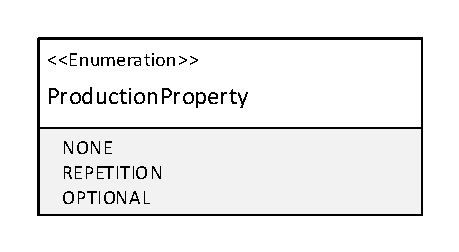
\includegraphics[width=.4\textwidth]{images/Concept_uml_data_types_production_property.pdf}
\caption{Production property data type UML class diagram}
\label{fig:ConceptProductionPropertyClassDiagram}
\end{figure}

A \textbf{production} is one of the production alternatives of a rule.
As can be seen in figure \ref{fig:ConceptProductionClassDiagram} it consists of a list of production elements and has a production property that is like the production property of the production\textunderscore element. Productions can also be nested.
Therefore, the list can also contain further productions. 

\begin{figure}[H]
\centering
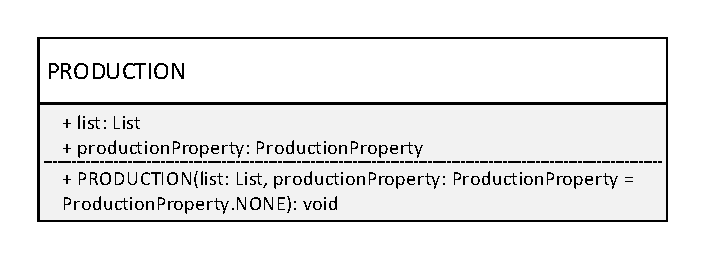
\includegraphics[width=.5\textwidth]{images/Concept_uml_data_types_production.pdf}
\caption{Production data type UML class diagram}
\label{fig:ConceptProductionClassDiagram}
\end{figure}

A \textbf{productions\textunderscore list} contains a list of productions where each production is one alternative in the description of an expression. 

The \textbf{XOR\textunderscore productions\textunderscore list} represents a productions\textunderscore list with multiple alternatives enclosed by parentheses. It contains a list of the alternate productions. Figure \ref{fig:ConceptProductionsListClassDiagram} shows the UML denotation of a productions\textunderscore list and a XOR\textunderscore productions\textunderscore list which is a an inherited productions\textunderscore list.

\begin{figure}[H]
\centering
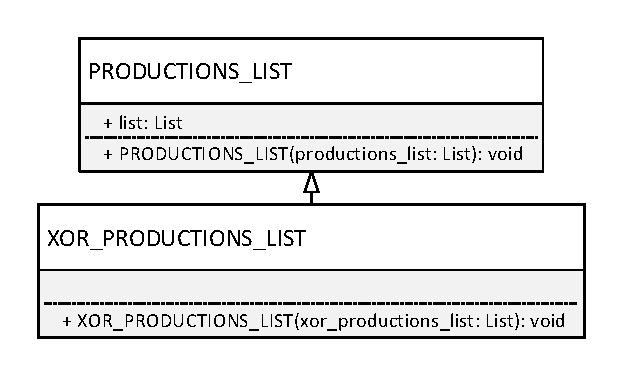
\includegraphics[width=.6\textwidth]{images/Concept_uml_data_types_productions_list.pdf}
\caption{Productions list data type UML class diagram}
\label{fig:ConceptProductionsListClassDiagram}
\end{figure}


The \textbf{grammar\textunderscore list} shown in figure \ref{fig:ConceptGrammarListClassDiagram} is the top level data structure. It contains a list of all rules that are in the TPTP syntax file.
This includes any type of rules (grammar, token, strict and macro) and comment blocks. 

\begin{figure}[H]
\centering
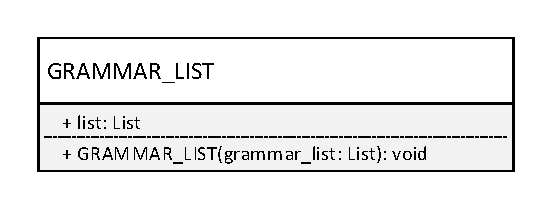
\includegraphics[width=.5\textwidth]{images/Concept_uml_data_types_grammar_list.pdf}
\caption{Grammar list data type UML class diagram}
\label{fig:ConceptGrammarListClassDiagram}
\end{figure}

\subsection{Disambiguation of  square brackets}\label{sec:ConceptDisambiguation}
As mentioned at the beginning of the parsing section, square brackets have different meanings depending on the rule type.
The idea to solve this problem is to treat all rules the same in the first processing step.
Square brackets are then interpreted as denoting the optional production property.
This production property is then selected for productions that are enclosed by square brackets for all types of rules.
In an additional processing step, after creating the grammar list each grammar and strict rule is iterated, exchanging the production property optional by the square bracket terminal symbols.
The output of the parser is a list of the rules and the comments from the \ac{TPTP} syntax file.

%
%To build the representative data structure, data types that represent the data stored in the \ac{TPTP} syntax have to be defined.
%The following section describes the data structure and data types that are used and created by the parser in the parsing process.
%
%%Atomic data types
%
%\subsubsection{Terminal symbol}
%The terminal symbol data type has one attribute, which is the name of the terminal symbol it represents.
%
%-todo Production Property
%
%\subsubsection{Nonterminal symbol}
%Analogue to the terminal symbol data type, the nonterminal symbol also has its name as an attribute.
%
%todo describe diagram
%\begin{figure}[H]
%\centering
%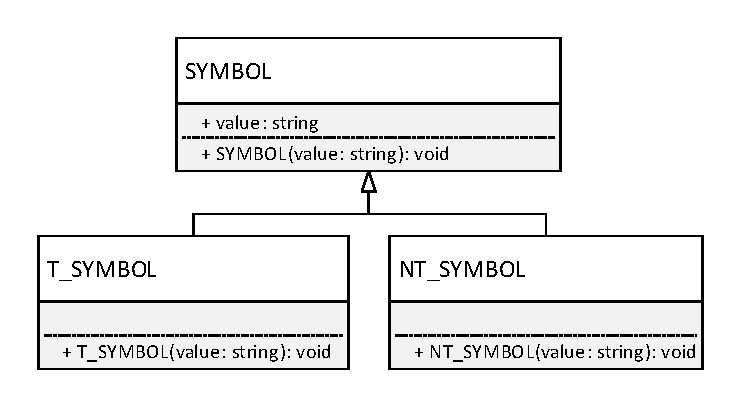
\includegraphics[width=.8\textwidth]{images/Concept_uml_data_types_symbols.pdf}
%\caption{Symbol data type UML class diagram}
%\label{fig:ConceptSymbolsClassDiagram}
%\end{figure}
%%Composite data types
%
%\subsubsection{Rules}
%%\subsubsection{Grammar Expression}
%A rule consists of the nonterminal symbol name which is produced, a production list and a position.
%The position denotes at which position in the \ac{TPTP} syntax the rule was listed.
%This information is needed to maintain the original order of the rules when printing the reduced syntax.\\
%For each rule type (see table \ref{tbl:ConceptTPTPProductionSymbols}) there is a data type.
%This means that grammar, token, strict and macro rule data types are introduced.\\
%Listing \ref{lst:ConceptParserGrammarExpression} contains an example of a line in a \ac{TPTP} syntax file that is represented by the grammar rule data type.
%The nonterminal symbol name which is produced is <$tff \textunderscore formula$>.  The production list consists of two productions, as can be seen in the listing.
%\begin{lstlisting}[basicstyle=\scriptsize	,caption= Grammar expression,label= lst:ConceptParserGrammarExpression]
%<tff_formula>          ::= <tff_logic_formula> | <tff_atom_typing
%\end{lstlisting}
%
%
%todo describe diagram
%\begin{figure}[H]
%\centering
%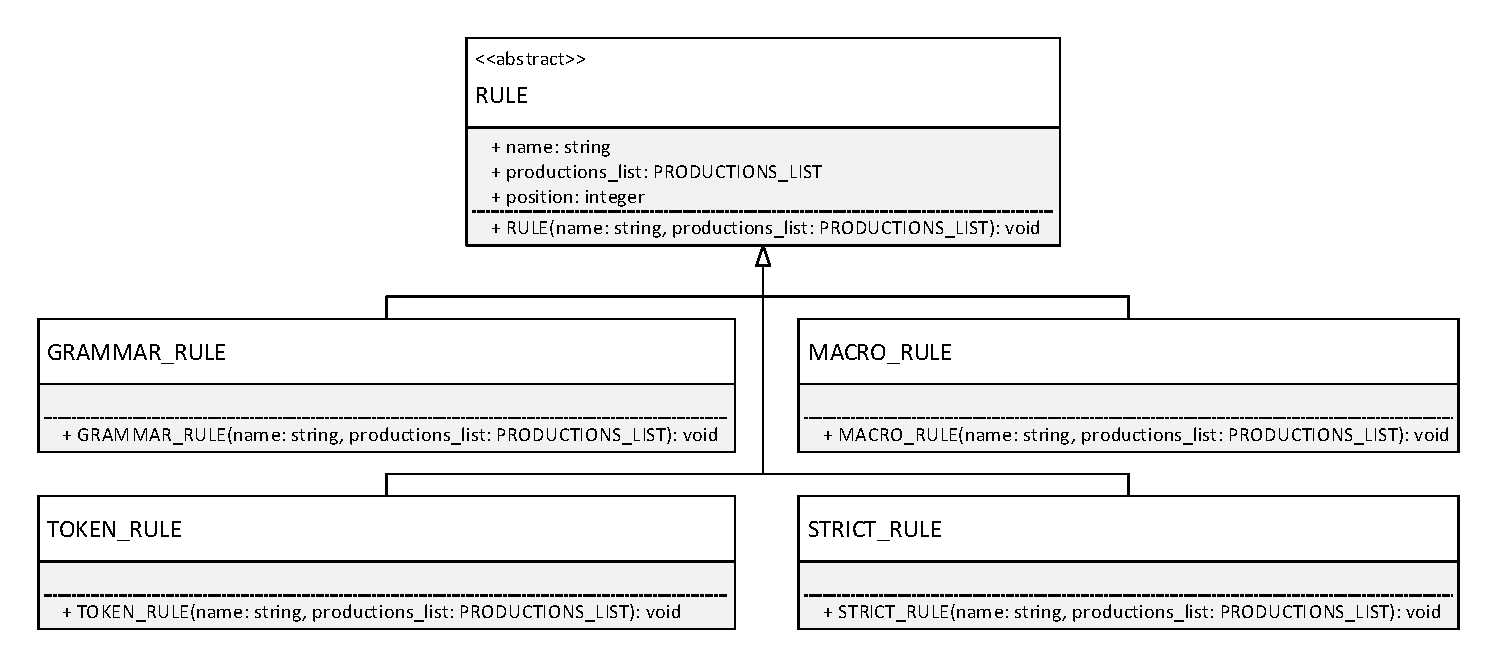
\includegraphics[width=1\textwidth]{images/Concept_uml_data_types_rules.pdf}
%\caption{Rule data type UML class diagram}
%\label{fig:ConceptRulesClassDiagram}
%\end{figure}
%
%\subsubsection{Comment block}
%A comment block is a list of consecutive comment lines.
%
%todo describe diagram
%\begin{figure}[H]
%\centering
%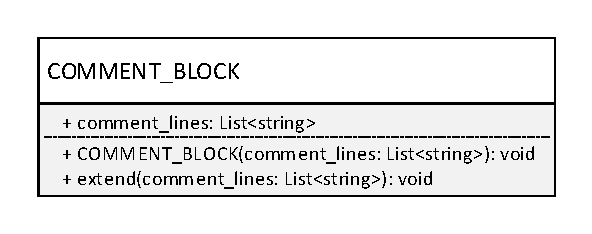
\includegraphics[width=.5\textwidth]{images/Concept_uml_data_types_comment_block.pdf}
%\caption{Comment block data type UML class diagram}
%\label{fig:ConceptCommentBlockClassDiagram}
%\end{figure}
%
%\subsubsection{Production element}
%A production element is either a terminal or nonterminal symbol. Additionally a production symbol has a production property.
%\begin{figure}[H]
%\centering
%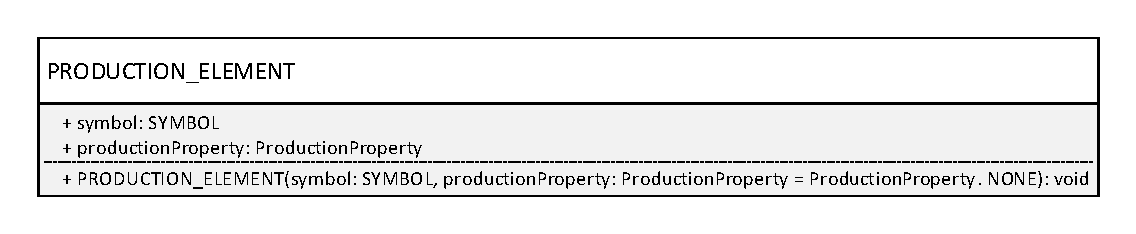
\includegraphics[width=.8\textwidth]{images/Concept_uml_data_types_production_element.pdf}
%\caption{Production element data type UML class diagram}
%\label{fig:ConceptProductionElementClassDiagram}
%\end{figure}
%
%\subsubsection{Production property}
%The production property can take one of three values and denotes whether a production is optional, can be repeated any number of times or does not have any special property.
%In the original \ac{TPTP} syntax file this was represented by square brackets or the repetition symbol.
%
%todo describe diagram
%\begin{figure}[H]
%\centering
%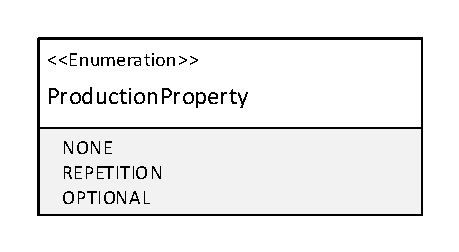
\includegraphics[width=.4\textwidth]{images/Concept_uml_data_types_production_property.pdf}
%\caption{Production property data type UML class diagram}
%\label{fig:ConceptProductionPropertyClassDiagram}
%\end{figure}
%
%\subsubsection{Production}
%A production is one production alternative specified in any expression.
%It consists of a list of production elements and has a production property. Productions can also be nested.
%Therefore the list can also contain further productions
%
%-show example
%\begin{figure}[H]
%\centering
%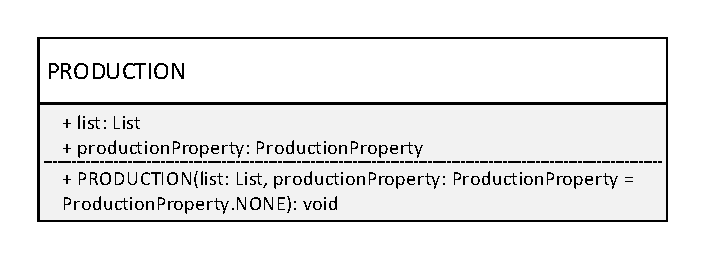
\includegraphics[width=.5\textwidth]{images/Concept_uml_data_types_production.pdf}
%\caption{Production data type UML class diagram}
%\label{fig:ConceptProductionClassDiagram}
%\end{figure}
%
%\subsubsection{Productions list}
%A productions list contains a list of productions where each production is one alternative in the description of an expression.
%
%
%\subsubsection{XOR Productions list}
%The XOR productions list represents multiple alternatives enclosed by parentheses. It contains a list of the alternate productions.
% 
% todo describe diagram
%\begin{figure}[H]
%\centering
%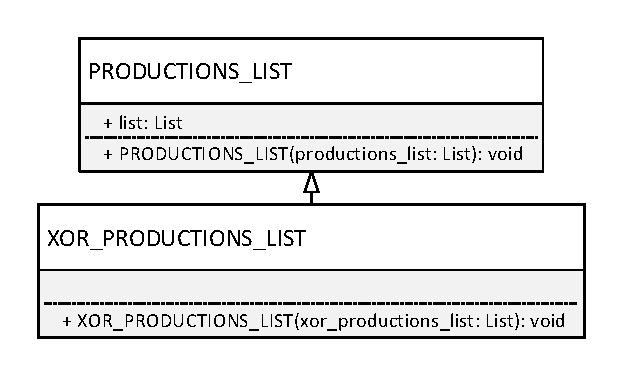
\includegraphics[width=.6\textwidth]{images/Concept_uml_data_types_productions_list.pdf}
%\caption{Productions list data type UML class diagram}
%\label{fig:ConceptProductionsListClassDiagram}
%\end{figure}
%
%\subsubsection{Grammar list}
%The grammar list is the top level data structure. It contains a list of all elements that were in the \ac{TPTP} syntax file.
%This includes any type of rules (grammar, token, strict and macro) and comment blocks.
%
%todo describe diagram
%\begin{figure}[H]
%\centering
%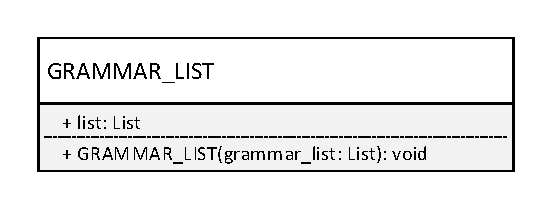
\includegraphics[width=.5\textwidth]{images/Concept_uml_data_types_grammar_list.pdf}
%\caption{Grammar list data type UML class diagram}
%\label{fig:ConceptGrammarListClassDiagram}
%\end{figure}
%\subsection{Production rules}
%When using the \ac{PLY} parser generator, production rules have to be defined.
%The rules describe how the tokens are to be processed.
%
%todo describe production rules

\section{Graph generation}\label{sec:ConceptGraphGeneration}

After parsing the \ac{TPTP} grammar is stored in a grammar list. The grammar list data structure is needed for modification and traversing.
The data structure that is used is a graph representing the grammar.

The non-terminal symbols in the \ac{TPTP} syntax are represented by a node class that has the following attributes (see also UML class diagram \ref{fig:ImplementationNTNodeUML}):
\begin{itemize}
\item value: name of non-terminal symbol
\item productions list: productions list of non-terminal symbol that has been created by the parser
\item rule type: rule type of non-terminal symbol
\item comment block: list of comments belonging to the non-terminal symbol
\item position: position of the production in the input file
\item children: nested list that contains the node of every non-terminal symbol that is part of the productions list grouped by productions in the productions list
\end{itemize}

Before generating the graph, a dictionary is created, that provides an efficient way accessing the nodes in order to build the grammar graph and also during the next steps of the sub-syntax generation.
This dictionary contains nodes constructed from the grammar list output by the parser that contains rules and comments. The combination of the nodes value and rule type form the unique key for each node. While constructing the dictionary, comments in the grammar list are associated to nodes using a heuristic that is described in section \ref{sec:ConceptMaintainingComments}.

Also, a new temporary start symbol is introduced.
This is necessary because one non-terminal symbol in the \ac{TPTP} syntax can be mapped to multiple nodes which the following example shows. \\
The example below shows the productions for the non-terminal symbol $\textless formula\textunderscore role\textgreater$.
Since this non-terminal symbol has multiple types of rules one node will be created for each rule type.
\begin{lstlisting}[caption= Productions of the non-terminal symbol $\textless formula\textunderscore role\textgreater$]
<formula_role>         ::= <lower_word>
<formula_role>         :== axiom | hypothesis | definition | assumption |
                           lemma | theorem | corollary | conjecture |
                           negated_conjecture | plain | type |
                           fi_domain | fi_functors | fi_predicates | unknown
\end{lstlisting}

If a non-terminal symbol that has multiple rule types is selected as the desired start symbol multiple nodes would represent that start symbol and therefore it would not be possible to select one node as the starting point of the graph generation.
To solve this problem, a temporary start symbol is introduced before generating the graph.
The temporary start symbol produces the start symbol that the user specified and is used as a starting point for the graph generation.
If the non-terminal symbol $\textless formula\textunderscore role\textgreater$ that was mentioned before would be selected as start symbol by the user, a temporary start symbol representing the rule
\begin{lstlisting}[caption= Rule of the temporary start symbol]
<start_symbol>         ::= <formula_role>
\end{lstlisting}
would be introduced.
This ensures that only one node is representing the start symbol that is used for graph generation.

Starting with the temporary start symbol, the graph is generated recursively. Iterating over each non-terminal symbol in the productions list of the start symbol, the corresponding nodes are identified. These nodes are then appended to the list of children of the start symbol. The identified children may again have children. This process is repeated until a node has no children because there are only terminal symbols in the productions list of a non-terminal symbol.

Since it is possible for a non-terminal symbol to be on the right side as well as on the left side of the same production rule, a node can also be its own child. To avoid revisiting the same node infinitely, it is checked whether a node already has children so that it will not be visited again. This also improves the performance of the tool as a non-terminal symbol that has already been visited will not be visited again independent of circular dependencies.

The following example shows a production rule and an abstract representation of the resulting list of children belonging to the node. Each production alternative is embedded in the children list of the node. %This is relevant for checking whether a non-terminal is terminating.

todo check listing below
\begin{lstlisting}[caption= Rule and resulting list of children]
Production rule:
<disjunction>  ::=  <literal> | <disjunction><vline><literal>
Output:
node.value: <disjunction>
node.ruleType: grammar
node.children: [[<literal>],[<disjunction>,<vline>,<literal>]]
\end{lstlisting}

\section{Control file}\label{sec:ConceptControlFile}

A format for specifying the desired start symbol and blocked productions is required.
Using a file-based configuration enables the user to store desired configurations so that a manual selection in the GUI is not necessary.
It is also essential for using the command line interface, because there manual selection is not possible.
The file should be human-readable and -editable.
The format should be easy to parse and allow to specify all necessary information.
This includes the desired start symbol and all production rules that should be blocked.
The proposed way to describe this information is to:

\begin{itemize}%[noitemsep]
	\item Define the desired start symbol in the first line.
	\item Define blocked productions grouped by the non-terminal symbol and rule type symbol, separating each group by a new line.
	First defining the non-terminal symbol, then the production symbol and after that the indexes of the alternatives that should be blocked (indexing starts at zero).
\end{itemize}
Identifying the production symbol is necessary because there are non-terminal symbols that have productions with more than one production symbol.\\
The example below contains a sample control file.
In this file, \textit{\textless TPTP\textunderscore file\textgreater} is specified as start symbol.
The second line indicates that the second grammar production alternative of the non-terminal symbol \textit{\textless TPTP\textunderscore input\textgreater} should be disabled.
Furthermore, the first, second, third and fifth grammar production alternative of the non-terminal symbol \textit{\textless annotated\textunderscore formula\textgreater} are said to be disabled in line 3.

\begin{lstlisting}[caption= Control file,label= lst:ConceptControlFile]
<TPTP_file>
<TPTP_input>,::=,1
<annotated_formula>,::=,0,1,2,5
\end{lstlisting}
This format is easy to parse and also enables users to specify their desired start symbols and blocked productions without having to use the GUI. The control file can also be generated from selections made by the user in the GUI.
It can be exported as a textfile.
When generating a sub-syntax from the user GUI selection a control file representing that selection is created internally as input for the next processing steps.

Specifying which production should be blocked, and not the ones should be kept, typically results in a significantly smaller file.
Storing the indexes of the productions that should be blocked offers that in case productions are renamed the control file would still be valid. On the other hand if productions are added or deleted from the original \ac{TPTP} syntax, the control file may have to be updated.

\section{Maintaining comments}\label{sec:ConceptMaintainingComments}

In the \ac{TPTP} syntax there are comments providing supplemental information about the language and its symbols and rules.
When generating a reduced grammar maintaining comments is desired. This means that comments from the original language specification should be associated with the rule they belong to and if the rule is still present in the reduced grammar, the comment should be as well.\\
Therefore, a mechanism has to be designed for the association of comments to grammar rules.

Listing \ref{lst:ConceptComment_tptp} features an example of a comment in a \ac{TPTP} syntax file. This comment begins with a \textit{Top of Page} line which, in the HTML version of the \ac{TPTP} syntax, contains a hyperlink which leads to the beginning of the syntax file.
The next line contains a relevant comment.\\
\begin{lstlisting}[language=none, basicstyle=\scriptsize	,caption= Comment in the \ac{TPTP} syntax,label= lst:ConceptComment_tptp]
%----Top of Page---------------------------------------------------------------
%----TFF formulae.
<tff_formula>          ::= <tff_logic_formula> | <tff_atom_typing> |
                           <tff_subtype> | <tfx_sequent>
\end{lstlisting}

The heuristic matching comments to rules takes these \textit{Top of Page} lines into account.
When there is a \textit{Top of Page} line in between comment lines it generally also splits comments semantically.
In listing \ref{lst:ConceptComment_tptp} can be seen that the comment in line 2 refers to the rule after.
Therefore it would be correct to associate the comment line after the \textit{Top of Page} line to the rule after.
Also, if there is one \textit{Top of Page} line in between multiple comment lines it is highly probable that the first part of the comment lines before the \textit{Top of Page} line refer to the rule before the comments and that the lines after the \textit{Top of Page} line refer to the rule after the comment lines.
This scenario can be seen in listing \ref{lst:Comment_split_example}.
The \textit{Top of Page} line is in line 28 and the comment lines before refer to the rule before.
The comment line after refers to the rule after that line.
\begin{lstlisting}[language=none, basicstyle=\scriptsize	,caption=Comment lines split by a \textit{Top of Page} line in the \ac{TPTP} syntax,label= lst:Comment_split_example]
<formula_role>         :== axiom | hypothesis | definition | assumption |
                           lemma | theorem | corollary | conjecture |
                           negated_conjecture | plain | type |
                           fi_domain | fi_functors | fi_predicates | unknown
%----"axiom"s are accepted, without proof. There is no guarantee that the
%----axioms of a problem are consistent.
%----"hypothesis"s are assumed to be true for a particular problem, and are
%----used like "axiom"s.
%----"definition"s are intended to define symbols. They are either universally
%----quantified equations, or universally quantified equivalences with an
%----atomic lefthand side. They can be treated like "axiom"s.
%----"assumption"s can be used like axioms, but must be discharged before a
%----derivation is complete.
%----"lemma"s and "theorem"s have been proven from the "axiom"s. They can be
%----used like "axiom"s in problems, and a problem containing a non-redundant
%----"lemma" or theorem" is ill-formed. They can also appear in derivations.
%----"theorem"s are more important than "lemma"s from the user perspective.
%----"conjecture"s are to be proven from the "axiom"(-like) formulae. A problem
%----is solved only when all "conjecture"s are proven.
%----"negated_conjecture"s are formed from negation of a "conjecture" (usually
%----in a FOF to CNF conversion).
%----"plain"s have no specified user semantics.
%----"fi_domain", "fi_functors", and "fi_predicates" are used to record the
%----domain, interpretation of functors, and interpretation of predicates, for
%----a finite interpretation.
%----"type" defines the type globally for one symbol; treat as $true.
%----"unknown"s have unknown role, and this is an error situation.
%----Top of Page---------------------------------------------------------------
%----THF formulae.
<thf_formula>          ::= <thf_logic_formula> | <thf_atom_typing> |
                           <thf_subtype> | <thf_sequent>
\end{lstlisting}

The flow chart in figure \ref{fig:ConceptMaintainingComments} shows the process of matching comment blocks, that are consecutive comment lines (see section \ref{sec:ConceptParserDataStructure}),  to rules.
First, the comment block is split into multiple separate comment blocks by using \textit{Top of Page} lines as separators.
\begin{itemize}%[noitemsep]
	\item If this results in no comment blocks the comment block consisted only of one line which was a \textit{Top of Page} line.
	Then no comment block has to be associated to a rule because \textit{Top of Page} lines are not relevant.
	\item If this results in one comment block, that means that no \textit{Top of Page} line was present in the comment block or that there was a \textit{Top of Page} line at the beginning or end of the comment block. The comment block is associated with the rule after, if the comment block is not at the end of the file.
	If it is at the end of the file, it is associated with the rule before, because no rule after exists.
	\item If this results in two comment blocks, one \textit{Top of Page} line was present in between comment lines.
	Then the comment block before the \textit{Top of Page} line is associated with the rule before when possible and the comment block after the \textit{Top of Page} line is associated with the rule after.
	If the original comment block was at the beginning of the file, both comment blocks resulting from splitting the original comment block are associated with the rule after.
	If the original comment block was at the end of the file, the comment blocks resulting from the split are associated with the rule before.
\end{itemize}
The case of three or more comment blocks after splitting the original comment block is not featured in the flow chart.
This case does not occur in the \ac{TPTP} syntax version 7.3.0.
Since it might occur in a future version of the \ac{TPTP} syntax it is handled by merging all comment blocks starting from the second and then following the procedure of two comment blocks in the flow chart in figure \ref{fig:ConceptMaintainingComments}.

\begin{figure}[H]
\centering
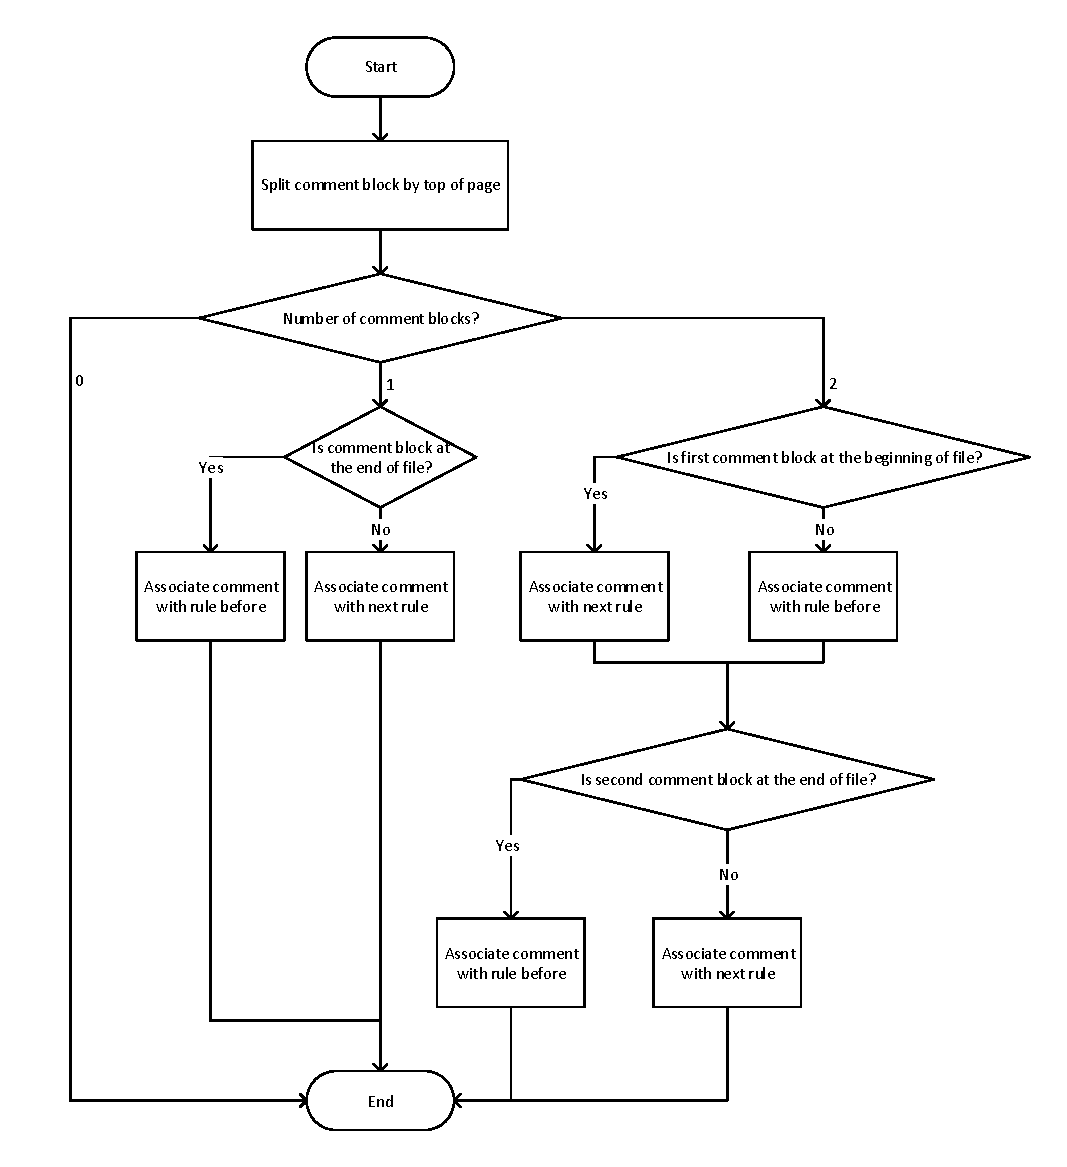
\includegraphics[width=1\textwidth]{images/Concept_maintaining_comments.pdf}
\caption{Maintaining comments flow chart}
\label{fig:ConceptMaintainingComments}
\end{figure}

\section{Extraction of a sub-syntax}\label{sec:ConceptExtractReducedGrammar}

This section covers the concept of how a sub-syntax is computed from the original syntax.
The original syntax is represented by a grammar graph (see section \ref{sec:ConceptGraphGeneration}) and the information on what part of the syntax to extract is described in a control file.
To extract a sub-syntax from the original grammar graph, four steps must be performed:
\begin{enumerate}%[noitemsep]
	\item The control file has to be parsed, in order to get information on the desired start symbol and which productions should be blocked.
	\item The blocked productions specified in the control file must be disabled and therefore the corresponding transitions must be removed from the grammar graph.
	\item The remaining part of the grammar that is terminating must be computed.
	\item From the part of the grammar that is terminating, non-reachable symbols must be removed.
\end{enumerate}

\subsection{Parsing a control file}\label{sec:ConceptParsingControlFile}

The control file provides the necessary information for the extraction of a sub-syntax.
The format of the control file is described in section \ref{sec:ConceptControlFile}. 
The start symbol is listed in the first line.
Every consecutive line contains a nonterminal symbol, the corresponding rule type symbol, and the indexes of the productions that should be blocked separated by comma.
The start symbol will be relevant in determining the remaining reachable part of the grammar (section \ref{sec:ConceptDerterminingRemainingReachable}) whereas the information on the productions that should be blocked will be needed in the next section.

\subsection{Removal of blocked productions}\label{sec:ConceptRemovingBlockedProductions}

In the control file, for each nonterminal symbol, productions should be modified, its name, rule type and the indexes of the productions that should be blocked are listed.
From all nodes, that are addressed (by nonterminal symbol name and rule type), the indexed productions are removed.
This includes deleting the corresponding element from the productions list and from the children list.

\subsection{Determination of the remaining terminating symbols}\label{sec:ConceptDerterminingRemainingTerminating}

After the desired productions have been deleted from the grammar graph, the next step is to remove the nonterminating symbols from the grammar graph.
First it must be determined which symbols are terminating and which are nonterminating.
Terminating nodes are found by iterating the nodes in the \textit{children\textunderscore list} of a node.
If the \textit{children\textunderscore list} is empty, the production only consists of terminal symbols.
If that is not the case, the node is terminating if all nodes in the \textit{children\textunderscore list} represent a non-terminal symbol which is terminating.
If a non-terminal symbol has multiple rule types, it is represented by multiple nodes. Also, if a non-terminal symbol with multiple rule types is in featured in a production, all nodes representing that non-terminal symbol are in the children list corresponding to this production. However, only one of the nodes needs to be terminating for the non-terminal symbol to be terminating.

After the terminating symbols have been determined, productions that contain a nonterminating symbol must be removed from the nodes of the grammar graph. Because some non-terminal symbols might have productions that contain nonterminating symbols, but also other productions that only contain terminating symbols, only the productions containing nonterminating symbols must be removed.

%After the desired productions have been deleted from the grammar graph, the next step is to remove the nonterminating symbols from the grammar graph.
%Non-terminating productions are productions in which at least one nonterminal symbol is non-terminating.
%First it must be determined which symbols are terminating and which are nonterminating.
%The terminating symbols can be determined recursively using dynamic programming techniques.
%The goal is to determine for each nonterminal symbol if it derives a terminating symbol. Only then it is a useful symbol since it is reachable and derives a terminating symbol todo reference
%Starting at the start symbol, the grammar graph is traversed. 
%
%-start with start symbol
%-traverse through graph and compute terminating symbols
%- store visited nodes to avoid infinite loops

\subsection{Determination of the remaining reachable symbols}\label{sec:ConceptDerterminingRemainingReachable}

After removing the productions specified in the control file it has to be determined which part of the grammar still remains reachable.
This is done by generating a new grammar graph starting from desired the start symbol.
When generating the new grammar graph, all from the start symbol reachable parts of the grammar will be added to the new grammar graph (see section \ref{sec:ConceptGraphGeneration}).
All nodes that are not part of the new grammar graph are not reachable and can therefore be removed. They are also removed from the nodes dictionary.

\section{Output generation}\label{sec:ConceptOutputGeneration}

Within \ac{Synplifier} a syntax is represented by a grammar graph.
To export sub-syntaxes that have been extracted from a grammar graph they have to be converted to the original form of a \ac{TPTP} syntax file. This process is described in the following subsection.
After that, measures to provide compatibility with the automated parser generator are discussed in section \ref{sec:ConceptAutomatedParserGenerator}.

\subsection{Create output from grammar graph}\label{sec:ConceptOutputGrammarGraph}

There are three steps necessary in order to convert a syntax represented by a grammar graph to the original \ac{TPTP} syntax file form. These steps are displayed in figure \ref{fig:ConceptOutputGrammarGraphProcedure}.

The first step is to traverse the grammar graph by iterating all nodes and getting a string representation of the nodes.
For creating the string representation, the Python string class is used (\url{https://docs.python.org/3/library/stdtypes.html#str}). The string class creates a string version of the object passed to the constructor.
To do that it calls the \textit{\textunderscore \textunderscore str \textunderscore \textunderscore ()} of the passed object, if the object provides that method.

In order to maintain the same order that rules have had in the original \ac{TPTP} syntax, the position of the nodes is saved together with the node string in a tuple. 
After generating all node string representations, in the second step all tuples are ordered based on their position. 

The ordered list of nodes strings is then, in the third step, written to a file and exported.
The node that represents the temporary start symbol is not printed as it does not belong to the \ac{TPTP} syntax. 
 
\begin{figure}[H]
\tikzstyle{decision} = [ diamond, draw, fill=blue!10, text width=4.5em, text badly centered, node distance=2cm, inner sep-0pt]  
\tikzstyle{block} = [ rectangle, draw, fill=blue!10, text width=10em, text badly centered, rounded corners, minimum height=4em]  
\tikzstyle{line} = [ draw, -latex']  
\tikzstyle{terminator} = [rectangle, draw, fill=blue!10, text width=10em, text badly centered, rounded corners, minimum height=4em]  
\begin{center}
\begin{tikzpicture}[node distance=5.5cm, auto]  
  \node [terminator]  (traverse)  {Traverse grammar graph and get nodes strings and positions};  
  \node [block, right of=traverse]  (order) {Order nodes strings by positions};  
  \node [terminator, right of=order] (store) {Store ordered nodes strings in file}; 

  \path [line] (traverse)  -- (order);  
  \path [line] (order) -- (store);  
\end{tikzpicture}
\end{center}
\caption{Procedure of generating a Syntax string representation from the grammar graph}
\label{fig:ConceptOutputGrammarGraphProcedure}
\end{figure}

\subsection{Automated parser generator compatibility}\label{sec:ConceptAutomatedParserGenerator}

The automated parser generator for the \ac{TPTP} syntax \cite{VS06} takes a \ac{TPTP} syntax file as input and creates a lex and yacc file corresponding to the specification in the input syntax.\\
In the \ac{TPTP} syntax version 7.3.0 there is a definition of the syntax of comments which is shown in listing \ref{lst:ConceptAutomatedParserGeneratorComment}.
\begin{lstlisting}[language=none, basicstyle=\scriptsize, caption=Comment syntax definition in the \ac{TPTP} syntax, label= lst:ConceptAutomatedParserGeneratorComment]
<comment>              ::- <comment_line>|<comment_block> 
<comment_line>         ::- [%]<printable_char>*
<comment_block>        ::: [/][*]<not_star_slash>[*][*]*[/]
<not_star_slash>       ::: ([^*]*[*][*]*[^/*])*[^*]*
<printable_char>       ::: .
\end{lstlisting}

However, this part of the syntax is not reachable from the start symbol $TPTP\textunderscore file$.
When constructing the grammar graph this part of the syntax is therefore removed.\\
Using a syntax file, in which the comment syntax is not present, with the automated parser generator results in an error because the comment symbol is not present in the lex specification but is referred to in a yacc rule.\\
There are two ways to include the comment syntax in the output of \ac{Synplifier} in order to be accepted by the automated parser generator.
Either making the \textit{<comment>} nonterminal symbol reachable by for example adding it as an alternative to \textit{<TPTP\textunderscore input>} which can be seen in listing \ref{lst:ConceptAutomatedParserGeneratorCommentReachable} or maintaining the comment syntax separately and adding it to the output syntax even though it is not reachable.
\begin{lstlisting}[language=none, basicstyle=\scriptsize, caption=Making the comment syntax reachable, label= lst:ConceptAutomatedParserGeneratorCommentReachable]
<TPTP_file>            ::= <TPTP_input>*
<TPTP_input>           ::= <annotated_formula> | <include> | <comment>
\end{lstlisting}

Both ways are supported by \ac{Synplifier}.\\
If the \textit{<comment>} nonterminal symbol is made reachable in the \ac{TPTP} syntax, the grammar graph generated by \ac{Synplifier} contains the comment syntax and no further action is necessary.\\
To add the comment syntax to the output if the \textit{<comment>} nonterminal symbol is not reachable is done by using an external configuration file that contains the syntax from listing \ref{lst:ConceptAutomatedParserGeneratorComment}.
From the syntax in this configuration file a separate grammar graph is generated. The output string that can be generated from this grammar graph is added to the output of \ac{Synplifier} when outputting a generated sub-syntax.

-Menu option

-make comment reachableto be tested

\section{GUI}\label{sec:ConceptGUI}

The graphical user interface is built using PyQt. Advantages of PyQT are that it offers a treeview that is used for displaying the grammar. In comparison to the standard Python tool kit Tkinter PyQt offers checkboxes in treeviews \cite{Tkinter} that are used for selecting blocked productions.

The menu of the GUI consists of five submenus.

\subsection{Import Menu}\label{sec:ConceptGUIImportMenu}

The $Import$ menu that can be seen in figure \ref{fig:import} provides the option to import a \ac{TPTP} syntax file in txt file format from local storage or to import the latest \ac{TPTP} syntax version from the \ac{TPTP} website.
The \ac{TPTP} syntax on the \ac{TPTP} project website is stored in a HTML format.
This file is downloaded and converted to plain text using the Beautiful Soup Python library \cite{BeautifulSoup}.

\begin{figure}[H]
\centering
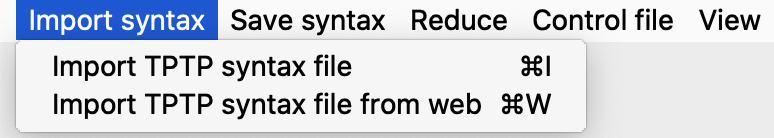
\includegraphics[width=.7\textwidth]{images/import.png}
\caption{Import menu}
\label{fig:import}
\end{figure}

After selecting a file for import a start symbol needs to be selected.
Starting with the start symbol a grammar graph is generated and the corresponding text displayed.
Each rule in the \ac{TPTP} grammar is a top element of the treeview and can be expanded to show the productions alternatives.
Right of the nonterminals name the rule type is displayed.
Comments that have been assigned to a rule are also displayed. An example of the imported \ac{TPTP} grammar is shown in figure \ref{fig:gui}.

\begin{figure}[H]
\centering
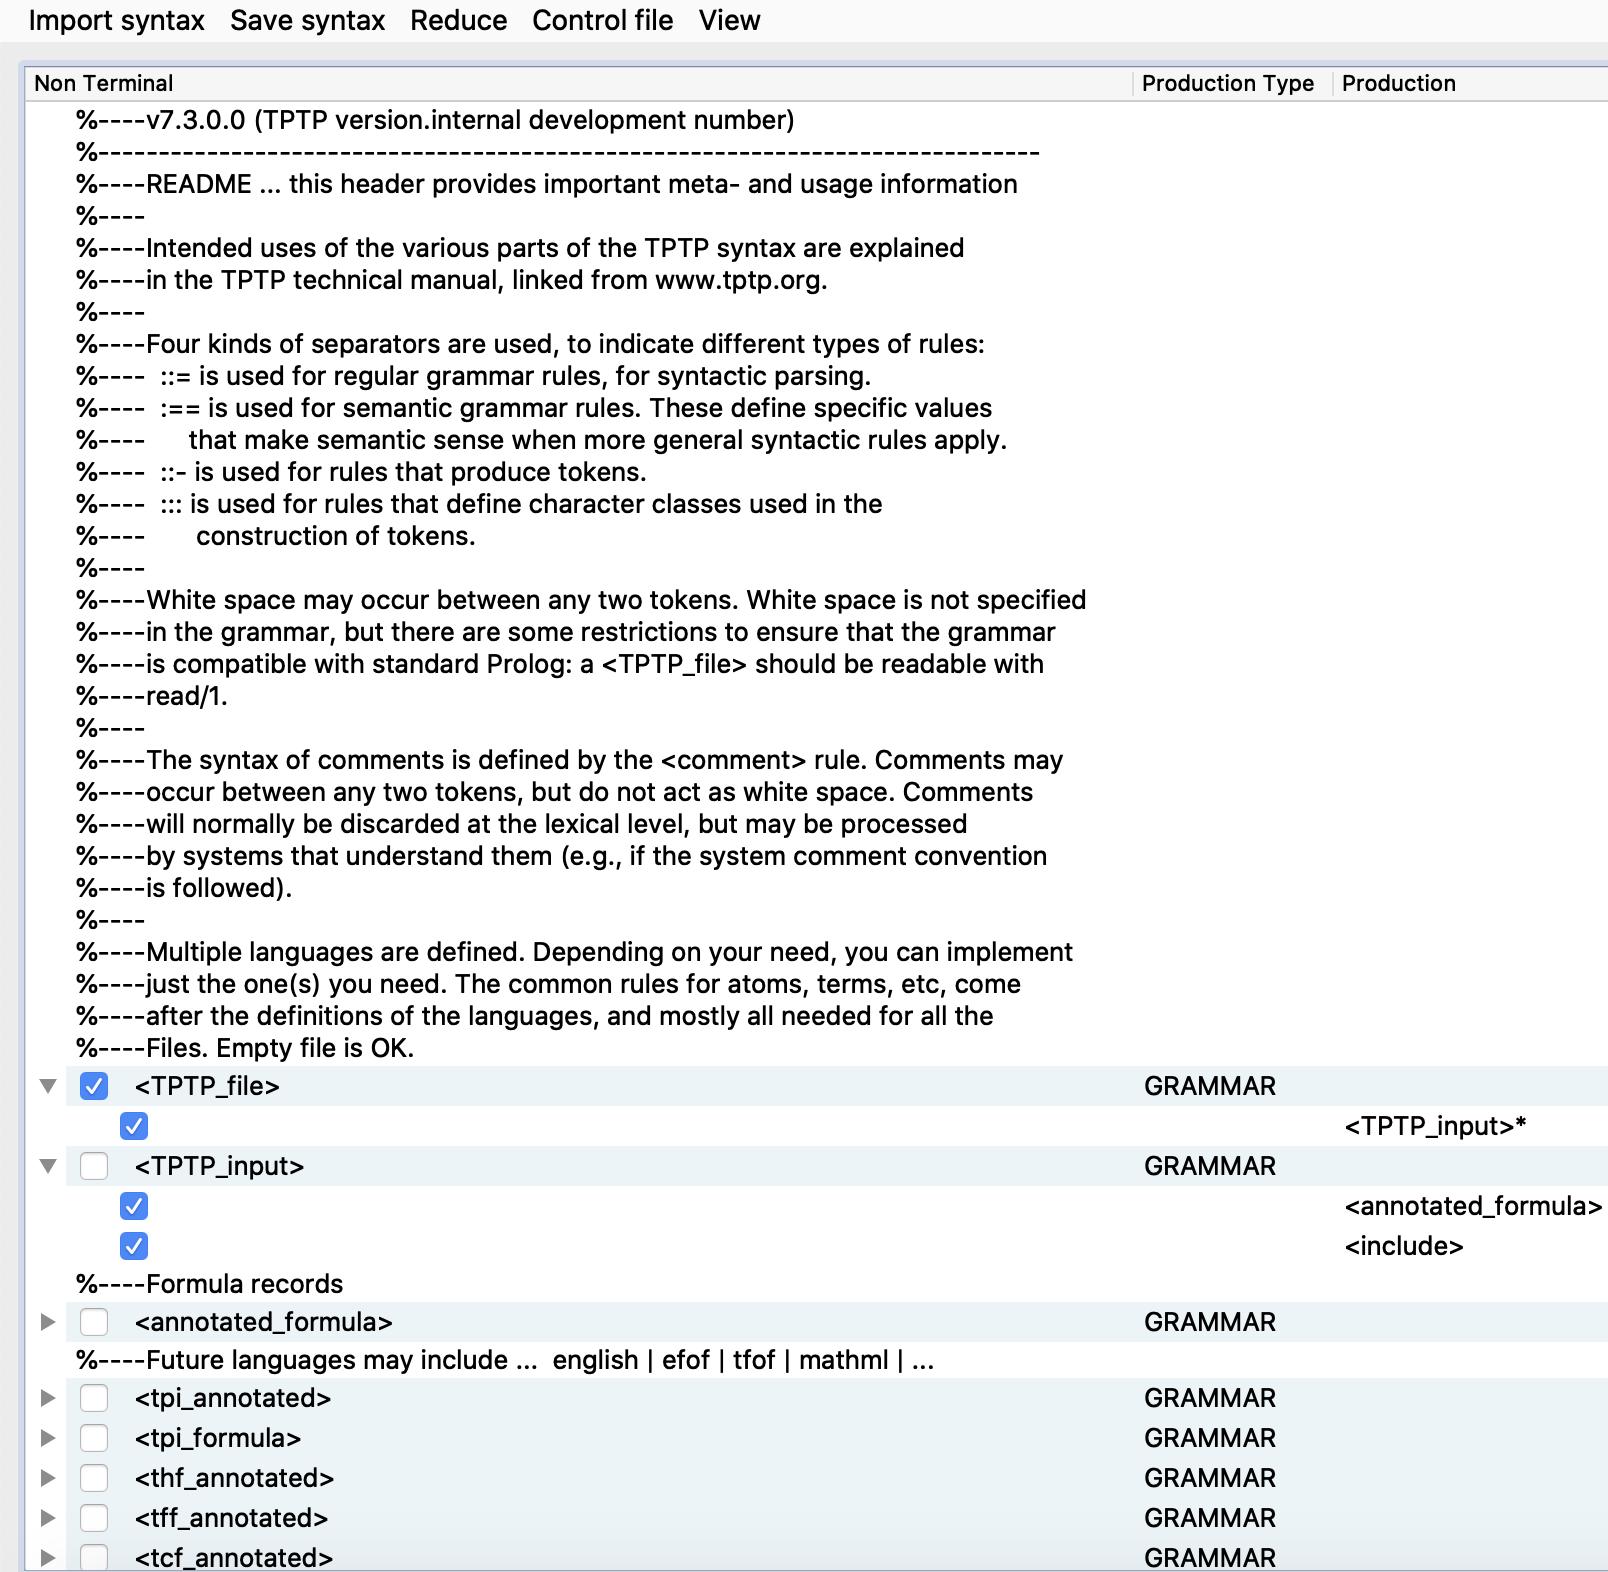
\includegraphics[width=1\textwidth]{images/gui.png}
\caption{GUI}
\label{fig:gui}
\end{figure}

\subsection{View Menu}\label{sec:ConceptGUIViewMenu}

The $View$ menu, shown in figure \ref{fig:view}, provides the possibility to toggle the display of comments to improve readability.

\begin{figure}[H]
\centering
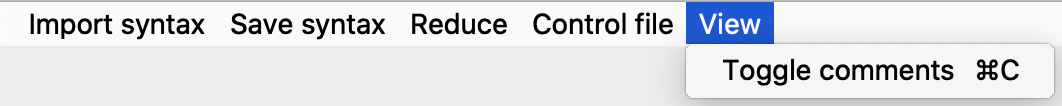
\includegraphics[width=.7\textwidth]{images/view.png}
\caption{View menu}
\label{fig:view}
\end{figure}

In order to extract a sub-syntax the user has to choose a new start symbol by checking one of the check boxes left of the nonterminal symbols name. By default, the start symbol that has been selected after importing the syntax is selected. For selecting blocked productions, the user has the choice of on the one hand expanding the rules and uncheck the checkboxes belonging to the productions the user wishes to block. On the other hand, the user can import a control file. If the user imports a control file, the checkboxes are set accordingly.

\subsection{Reduce Menu}\label{sec:ConceptGUIReduceMenu}

In the $Reduce$ menu that can be seen in figure \ref{fig:reduce} the user can reduce the syntax according to his selections. The syntax is reduced and the reduced syntax is displayed afterwards. The rules maintain the same order as in the original \ac{TPTP} syntax.

\begin{figure}[H]
\centering
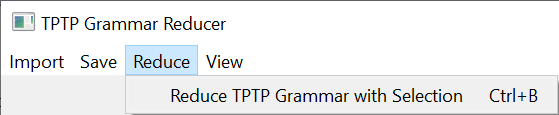
\includegraphics[width=.7\textwidth]{images/reduce.png}
\caption{Reduce menu}
\label{fig:reduce}
\end{figure}

\subsection{Save syntax Menu}\label{sec:ConceptGUISaveSyntaxMenu}

In the $Save\;syntax$ menu that is shown in figure \ref{fig:save} the user can reduce the syntax based on his GUI selection or an imported control file. The difference between the reduce option and the save menu is that the save menu saves the generated reduced syntax to local storage and does not display it. If the user wishes that the $\textless comments\textgreater$, which is necessary for using the automated parser generator, production is including in the reduced syntax the user has the option to save the reduced syntax with the $\textless comment\textgreater$ production.

\begin{figure}[H]
\centering
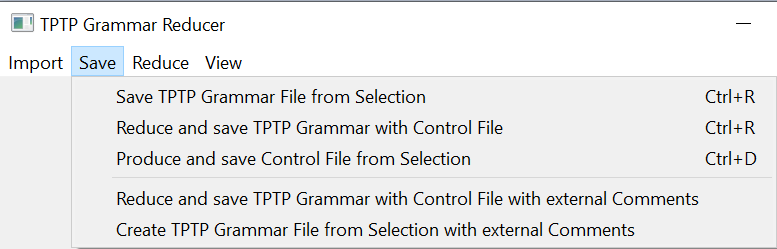
\includegraphics[width=.7\textwidth]{images/save.png}
\caption{Save menu}
\label{fig:save}
\end{figure}

\subsection{Control file Menu}\label{sec:ConceptGUIControlFileMenu}

The $Control\;file$ menu shown in figure \ref{fig:ControlFileMenu} gives the user the option to import a control file instead of blocking productions manually. If the user imports a control file, the checkboxes are set accordingly.
The user also has the option of generating a control file based on his GUI selection. This is particularly helpful if the users uses the same blocked productions multiple times. This way the user can use the import control file option later instead of selecting the blocked productions in the GUI.

\begin{figure}[H]
\centering
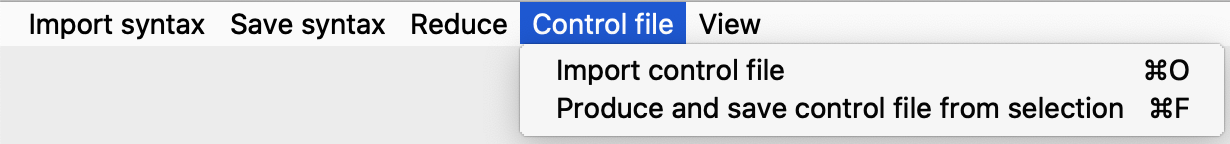
\includegraphics[width=.7\textwidth]{images/control_file_menu.png}
\caption{Control file menu}
\label{fig:ControlFileMenu}
\end{figure}

\section{Command-line interface}\label{sec:ConceptCommandLineInterface}

In addition to the GUI the software tool offers a command-line interface to provide the means for convenient automation of sub-syntax extraction.
It takes a \ac{TPTP} syntax file and a control file as input and outputs the resulting sub-syntax.
It is implemented using the Python module argparse\footnote{\url{https://docs.python.org/3/library/argparse.html}}, which provides a framework for creating command-line argument parsers.\\
The table below provides an overview about the implemented command-line arguments.
The syntax file location and the control file location have to be specified.
Specifying an output path and filename is optional, by default the output filename will be \textit{output.txt}.
The $-ex$ flag enables additional output of the comment syntax (see section \ref{sec:ConceptAutomatedParserGeneration}).
Additionally, the help description can be opened by using the \textit{-h} option.
\begin{table}[H]
\centering
\caption{Command-line interface parameters}
\begin{adjustbox}{width=1\textwidth, center=\textwidth}
\renewcommand{\arraystretch}{2}
\begin{tabular}{llll}
\textbf{Name} & \textbf{Short form} & \textbf{Default} & \textbf{Description}\\\hline
-{}-grammar & -g & None & \ac{TPTP} syntax file path and filename\\
-{}-control & -c & None &  Control file path and filename\\
-{}-output & -o & output.txt & Output file path and filename (optional)\\
-{}-external\textunderscore comment & -ex & False & Flag to include external comment syntax (optional)
\end{tabular}
\end{adjustbox}
\label{tbl:ImplementationCommandLineParameters}
\end{table}
The implementation of the command-line interface is described in section \ref{sec:ImplementationCommandLineInterface}.
More complex actions like control file generation can be done more comfortably by using GUI which is why this is not a feature of the command-line interface.\\
The design decision to separate the GUI from the command-line interface (see section \ref{sec:ConceptProposedArchitecture}) has the advantage that if a user chooses to solely use the command-line interface, it is not necessary to install the library used in GUI implementation (PyQt 5).

\section{Counting the number of rules in the TPTP syntax}\label{sec:ConceptCountR}

\subsubsection{Counting rules in a grammar graph}\label{sec:ConceptCountR}

-count rules to compare syntax sizes and for statistics/information

-count rules and productions

-count rules by counting nodes in grammar graph and count productions by counting number of productions list elements of all nodes

-count by traversing nodes in graph

-in addition counting only grammar rules

-print number of rules in console on import or sub-syntax generation

-since grammar graph only contains reachable and terminating symbols, not full TPTP syntax can be counted

\subsection{Counting rules in the original syntax}\label{sec:ConceptCountR}

-to count full TPTP syntax (including non reachable and terminating symbols)

-necessary to better compare original TPTP syntax to generated sub-syntaxes

-create a separate script, which uses parser and grammar list

-and count that
